\documentclass[presentation,aspectratio=43, 10pt]{beamer}
\usepackage{pifont}
\newcommand{\cmark}{\ding{51}}
\newcommand{\xmark}{\ding{55}}

\usepackage{booktabs}
\titlegraphic{\hfill
\includegraphics[height=1.25cm]{durham-logo}}
\usepackage{appendixnumberbeamer}
\usepackage{amsmath}
\usepackage{amssymb}
\usepackage{mathtools}
\usepackage{hyperref}
\usepackage{xspace}
\newcommand{\arxivlink}[2]{{\texttt{arXiv:\,\href{https://arxiv.org/abs/#1}{#1\,[#2]}}}}

\newcommand{\honev}{\ensuremath{{H}^1(\Omega; \mathbb{R}^d)}\xspace}
\newcommand{\ltwov}{\ensuremath{{L}^2(\Omega; \mathbb{R}^d)}\xspace}
\newcommand{\ltwo}{\ensuremath{{L}^2(\Omega)}\xspace}
\newcommand{\inner}[1]{\left\langle #1 \right \rangle}
\DeclareMathOperator{\Adj}{Adj}

\usepackage{pgfplots}
\usepackage{pgfplotstable}
\usepgfplotslibrary{dateplot}
\usepackage{minted}
\usepackage[url=false,
doi=true,
isbn=false,
style=authoryear,
maxnames=5,
giveninits=true,
uniquename=init,
backend=biber]{biblatex}
\renewcommand{\bibfont}{\fontsize{7}{7}\selectfont}
\addbibresource{references.bib}

\setlength{\bibitemsep}{1ex}
\setlength{\fboxsep}{1pt}

\renewbibmacro{in:}{}
\DeclareFieldFormat[article]{volume}{\textbf{#1}}
\DeclareFieldFormat{doi}{%
  doi\addcolon%
  {\scriptsize\ifhyperref{\href{http://dx.doi.org/#1}{\nolinkurl{#1}}}
    {\nolinkurl{#1}}}}
\AtEveryBibitem{%
\clearfield{pages}%
\clearfield{issue}%
\clearfield{number}%
}

\DeclareMathOperator{\grad}{grad}
\let\div\relax
\DeclareMathOperator{\div}{div}
\DeclareMathOperator{\curl}{curl}
\DeclareMathOperator{\range}{range}
\DeclareMathOperator{\sym}{sym}
\usetheme{metropolis}
\setbeamertemplate{title graphic}{
  \vbox to 0pt {
    \vspace*{1em}
    \inserttitlegraphic%
  }%
  \nointerlineskip%
}
\metroset{background=light,progressbar=frametitle,numbering=counter,block=fill}

% https://www.dur.ac.uk/marketingandcommunications/marketing/branding/colourpalette/
% Most of these are indistinguishable to those suffering colour blindness
\definecolor{purple}{HTML}{68246D}
\definecolor{blue}{HTML}{002A41}
\definecolor{red}{HTML}{BE1E2D}
\definecolor{cyan}{HTML}{00AEEF}
\definecolor{yellow}{HTML}{FFD53A}

\setbeamercolor{normal text}{
  fg=black,
  bg=white
}
\setbeamercolor{alerted text}{
  fg=red
}
\setbeamercolor{example text}{
  fg=blue
}

\setbeamercolor{palette primary}{%
  use=normal text,
  fg=normal text.bg,
  bg=purple,
}

\usetheme{metropolis}

\author{Lawrence Mitchell}
\institute{
  Department of Computer Science, Durham University\\
  \texttt{lawrence.mitchell@durham.ac.uk}}

\title{Beyond the ad-hoc: exploiting structure in mesh-based PDE libraries}

\usepackage{tikz}
\usetikzlibrary{trees,calc,positioning}
\usetikzlibrary{shapes, shapes.geometric}
\usetikzlibrary{arrows,chains,positioning,fit,backgrounds,calc,shapes,
  shadows,scopes,decorations.markings,plotmarks}

\newcommand*{\tettextsize}{\footnotesize}
\tikzstyle{line} = [draw, -, thick]
\tikzstyle{nodraw} = [draw, fill, circle, minimum width=0pt, inner sep=0pt]
\tikzstyle{sieve} = [line, circle, font=\tettextsize, inner sep=0pt,
  minimum size=12pt]

\tikzstyle{cell} = [sieve, fill=blue!60]
\tikzstyle{facet} = [sieve, fill=green!35]
\tikzstyle{edge} = [sieve, fill=red!35]
\tikzstyle{vertex} = [sieve, fill=blue!35]

% https://tex.stackexchange.com/questions/27171/padded-boundary-of-convex-hull
\newcommand{\convexpath}[2]{
  [
  create hullcoords/.code={
    \global\edef\namelist{#1}
    \foreach [count=\counter] \nodename in \namelist {
      \global\edef\numberofnodes{\counter}
      \coordinate (hullcoord\counter) at (\nodename);
    }
    \coordinate (hullcoord0) at (hullcoord\numberofnodes);
    \pgfmathtruncatemacro\lastnumber{\numberofnodes+1}
    \coordinate (hullcoord\lastnumber) at (hullcoord1);
  },
  create hullcoords
  ]
  ($(hullcoord1)!#2!-90:(hullcoord0)$)
  \foreach [
  evaluate=\currentnode as \previousnode using \currentnode-1,
  evaluate=\currentnode as \nextnode using \currentnode+1
  ] \currentnode in {1,...,\numberofnodes} {
    let \p1 = ($(hullcoord\currentnode) - (hullcoord\previousnode)$),
    \n1 = {atan2(\y1,\x1) + 90},
    \p2 = ($(hullcoord\nextnode) - (hullcoord\currentnode)$),
    \n2 = {atan2(\y2,\x2) + 90},
    \n{delta} = {Mod(\n2-\n1,360) - 360}
    in
    {arc [start angle=\n1, delta angle=\n{delta}, radius=#2]}
    -- ($(hullcoord\nextnode)!#2!-90:(hullcoord\currentnode)$)
  }
}

\graphicspath{{./\jobname.figures/}{../pictures/}}
\date{4 June 2019}
\begin{document}

\maketitle

% \begin{abstract}
%   Many mesh-based simulations occur one meshes with some regular
%   structure. Examples include, but are not limited to: composite
%   macro-elements and high continuity spline discretisations; regular
%   refinement in geometric multigrid; structured mesh extrusion (common
%   in ocean, ice sheet, and atmospheric modelling); and octree-like
%   AMR.

%   Typically, library developers might implement one (or more) of these
%   driven by particular application requirements: in the Firedrake
%   project we have an ad-hoc mechanism to handle the case of extruded
%   meshes.

%   An, I think, unanswered question is how to handle this kind of
%   structure in meshes in a composable way. For example, what if I want
%   a macro-element on an extruded mesh: I should exploit both kinds of
%   structure, but does this necessitate handling that case specially?
%   What if I want to try out different ways of traversing the
%   structured part to get better cache efficiency, or vectorisation
%   opportunities?

%   I will present some nascent ideas on developing symbolic and
%   code-generation abstractions for talking about structure in meshes,
%   hopefully in a way that removes the need to code the cartesian
%   product of all possible combinations by hand.

%   These are joint musings with Christian Engwer (Muenster), and David Ham
%   and Paul Kelly (Imperial).
% \end{abstract}


\begin{frame}
  \frametitle{Memory bandwidth is a precious commodity}
  \pgfplotstableset{
    create on use/ai/.style={
      create col/expr={\thisrow{GFLOPs}/\thisrow{Bandwidth}}}}
  \begin{tikzpicture}
    \begin{axis}[
      height=0.7\textheight,
      legend pos=outer north east,
      legend style={name=legend, cells={anchor=west, align=left, font=\footnotesize}},
      date coordinates in=x,
      date ZERO=2007-12-31,
      xticklabel style={rotate=90},
      xtick={2007-12-31,2008-12-31,2009-12-31,2010-12-31,2011-12-31,2012-12-31,
        2013-12-31,2014-12-31,2015-12-31,2016-12-31,2017-12-31},
      xticklabel={YE \year},
      ylabel near ticks,
      ylabel={DP FLOP/Byte}]
      \addplot+ table[x=Year, y=ai, col sep=comma]
      {\jobname.figures/data-intel.txt};
      \addlegendentry{Intel CPUs};
      \addplot+ table[x=Year, y=ai, col sep=comma]
      {\jobname.figures/data-intel-phi.txt};
      \addlegendentry{Intel Phi};
      \addplot+ table[x=Year, y=ai, col sep=comma]
      {\jobname.figures/data-nvidia.txt};
      \addlegendentry{Nvidia GPUs};
    \end{axis}
    \node [below=0cm of legend.south west, anchor=north west, text width=3cm] {{\tiny Data from Karl Rupp
      \url{github.com/karlrupp/cpu-gpu-mic-comparison}
      licensed under CC-BY.}};
  \end{tikzpicture}
\end{frame}

\begin{frame}[fragile]
  \frametitle{Typical mesh-based code}
  \begin{block}{Residual evaluation}
\begin{minted}[fontsize=\scriptsize]{python}
  ulocal <- global_to_local(uglobal)
  foreach element in mesh:
      uelement <- local_to_element(ulocal)
      relement <- compute_on_local(uelement)
      rlocal <- element_to_local(relement)
  rglobal <- local_to_global(rlocal)
\end{minted}
  \end{block}
  \begin{itemize}
  \item Cannot avoid moving field data
  \item \verb|local_to_element| uses topology of mesh (element->dof
    map)
  \item Can I avoid moving data for this?
  \end{itemize}
\end{frame}
\begin{frame}
  \frametitle{Idea: exploit structure}
  \begin{definition}[Unstructured mesh $\mathbb{U}$]
    Relationship between mesh entities provided by explicit
    enumeration.

    $\Rightarrow$ need to store relationship in arrays: data movement.
  \end{definition}
  \begin{definition}[Semi-structured mesh $\mathbb{U} \otimes \mathbb{S}$]
    Relationship between mesh entities sometimes available through
    closed form expression.
  \end{definition}
  \begin{definition}[Structured mesh $\mathbb{S}$]
    Relationship between mesh entities provided by closed form
    arithmetic expression

    $\Rightarrow$ less data movement
  \end{definition}
\end{frame}
\begin{frame}
  \frametitle{Examples}
  \begin{overlayarea}{\textwidth}{0.9\textheight}
    \begin{onlyenv}<1>
      \begin{block}{Extruded meshes}
        Often used in atmosphere, ocean, and ice sheet modelling. One
        structured direction.

        \begin{center}
          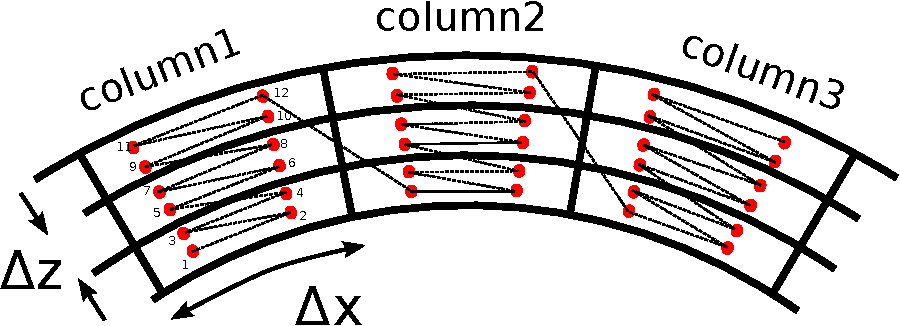
\includegraphics[height=0.4\textheight]{columndofs}
        \end{center}
      \end{block}
    \end{onlyenv}
    \begin{onlyenv}<2>
      \begin{block}{Barycentric refinement}
        Used for stability for Scott-Vogelius element pair,
        macro-element construction for $C^1$ elements.
        \begin{center}
          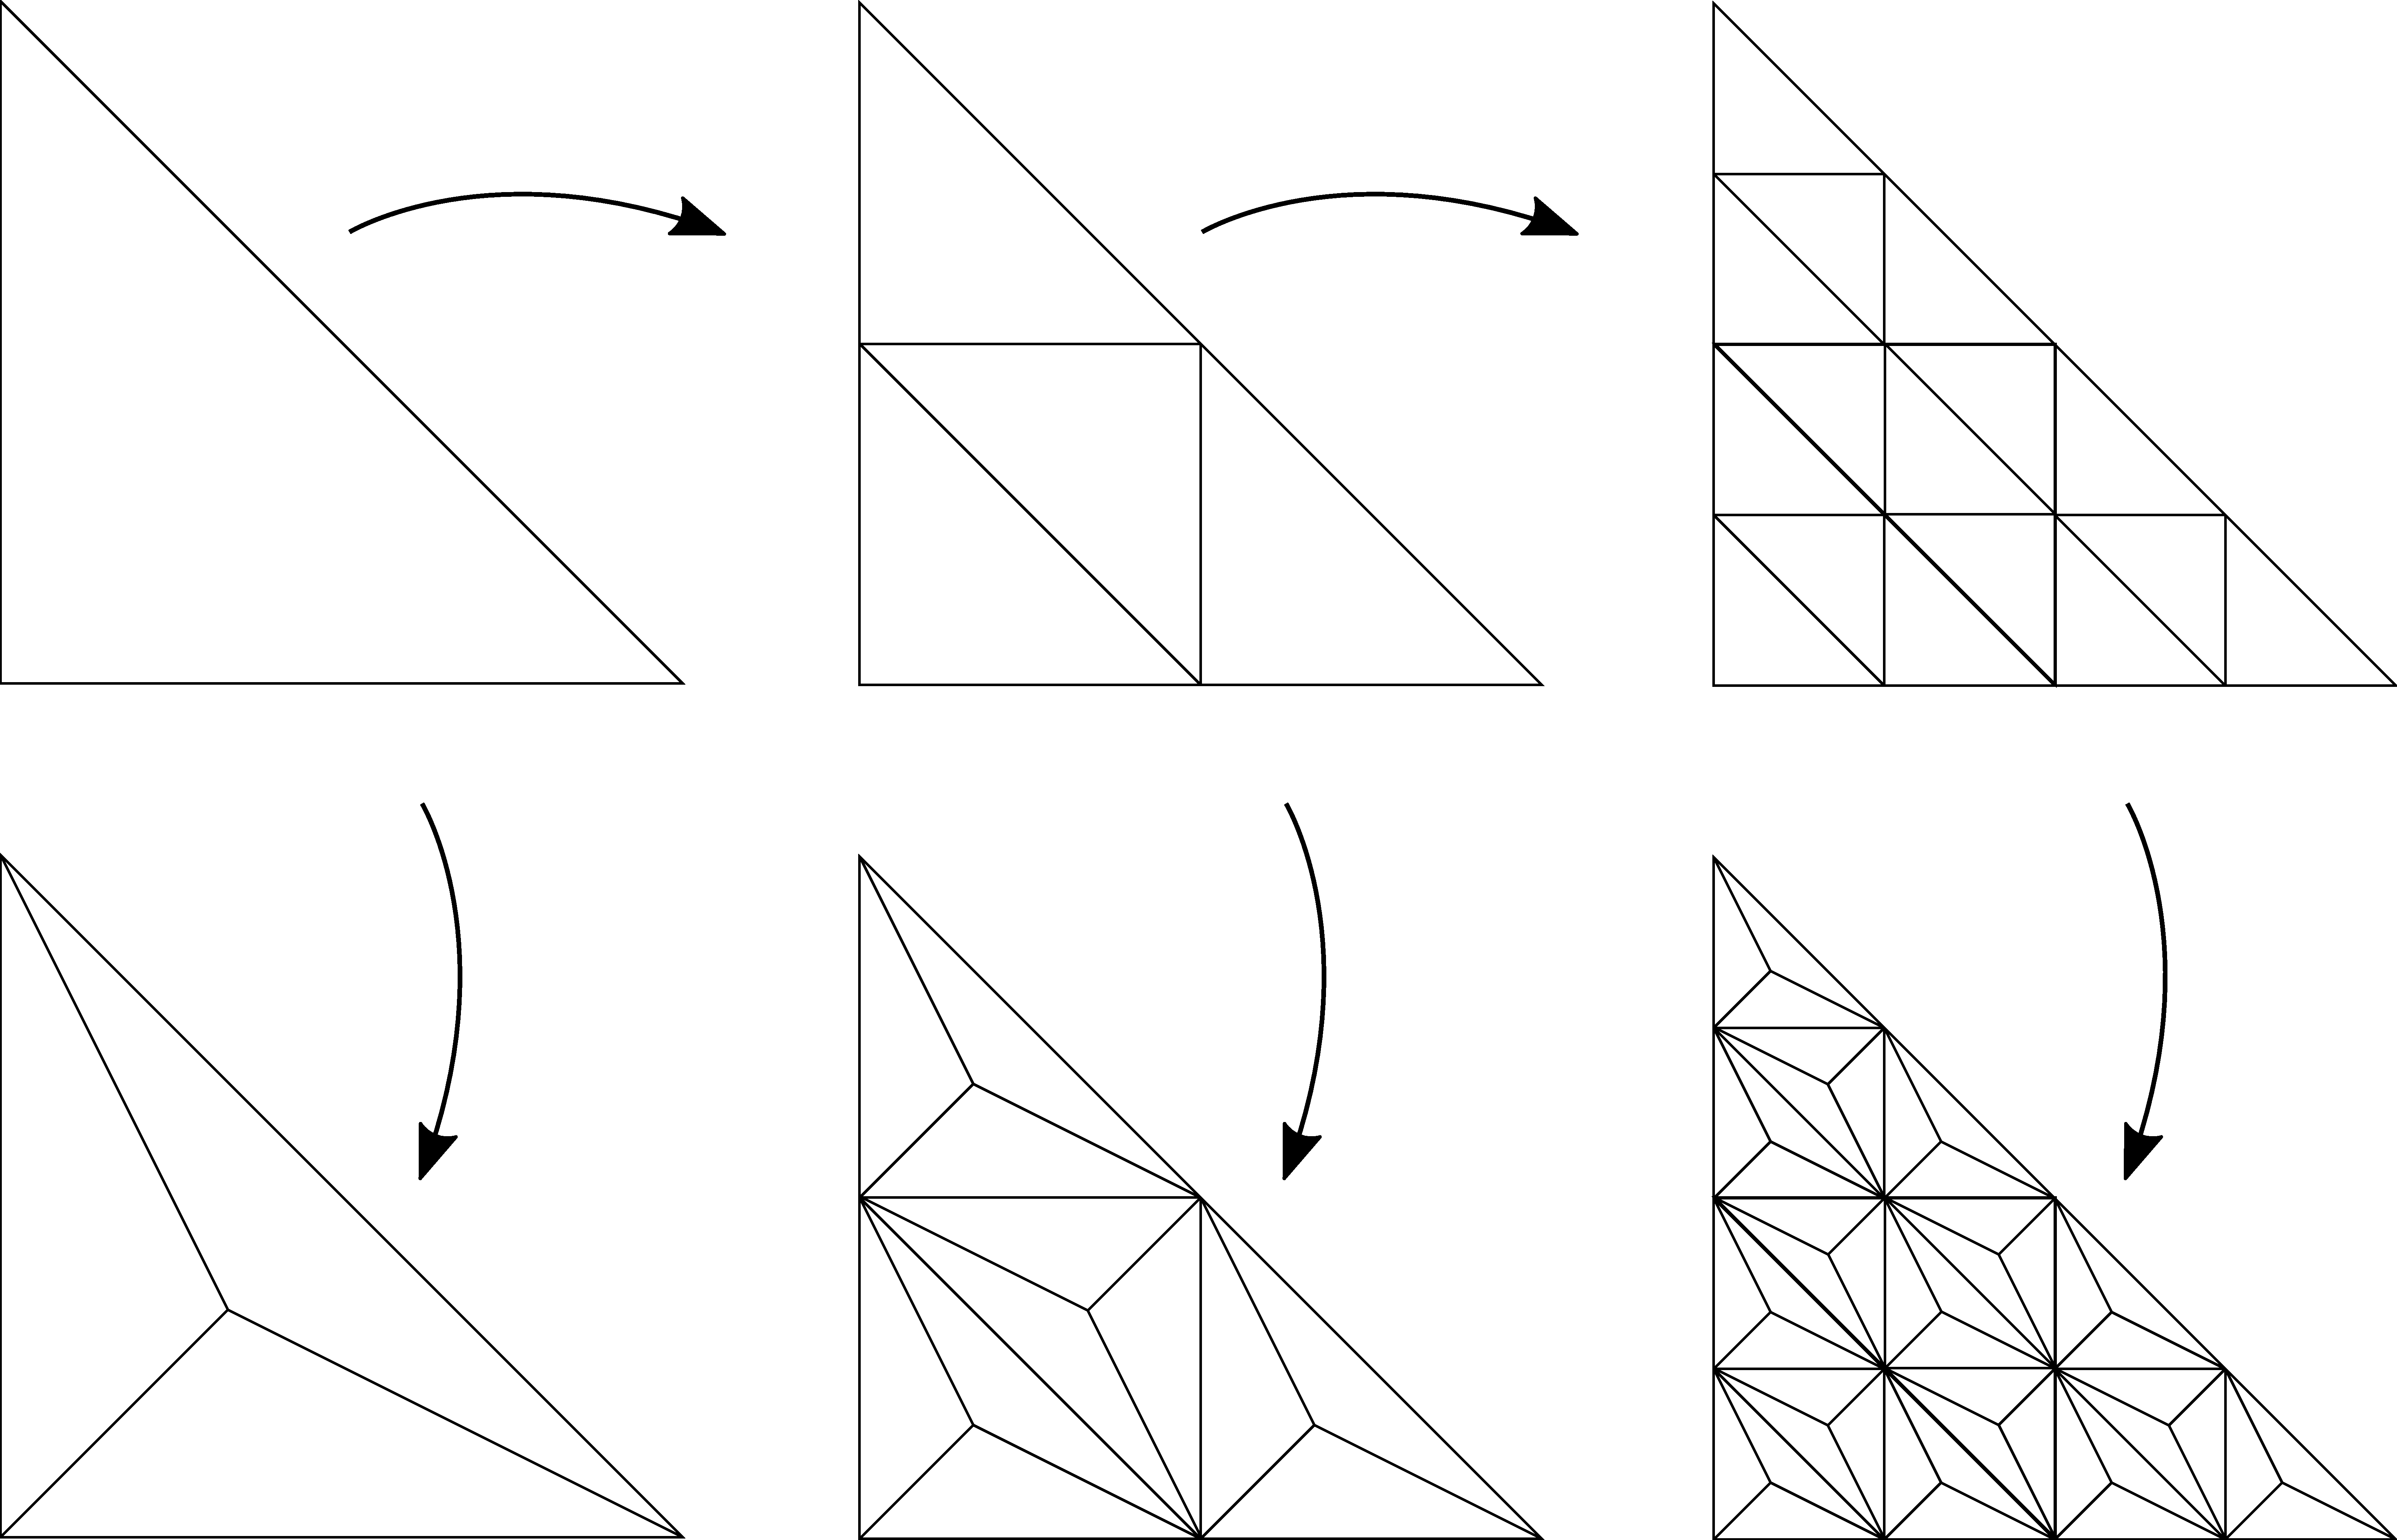
\includegraphics[height=0.6\textheight]{baryhierarchy}
        \end{center}
      \end{block}
    \end{onlyenv}
  \end{overlayarea}
\end{frame}
\begin{frame}
  \frametitle{Some motivation: extruded meshes}
  \begin{columns}
    \begin{column}{0.6\textwidth}
      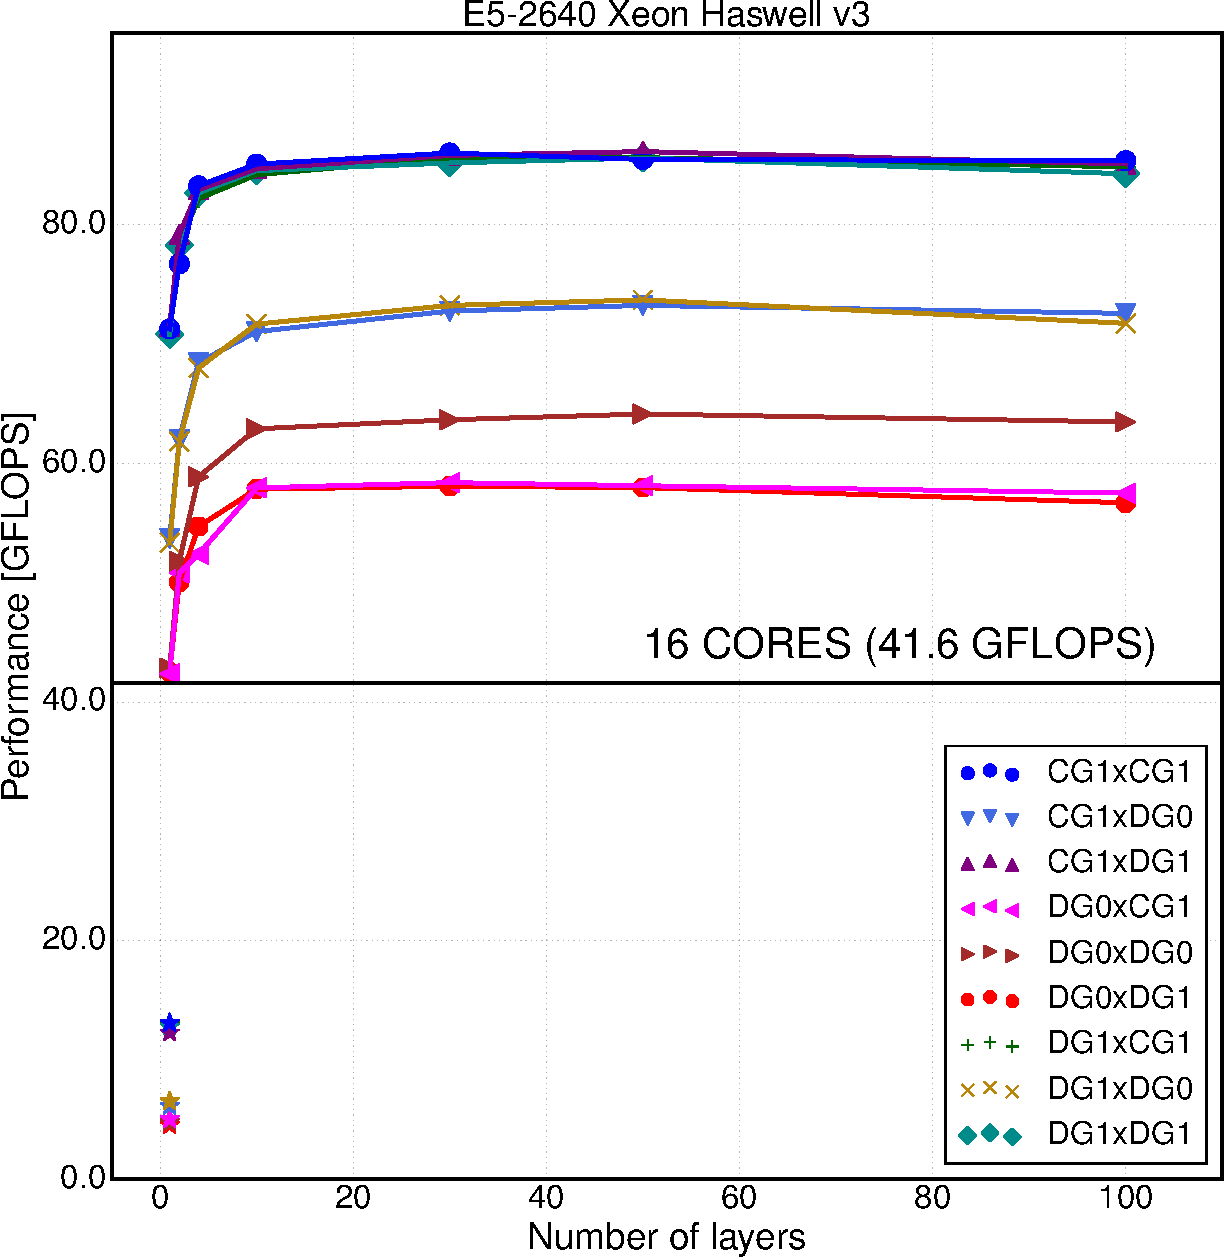
\includegraphics[height=0.7\textheight]{FRHS-32-2}
    \end{column}
    \hspace{-1em}
    \begin{column}{0.45\textwidth}
      \begin{itemize}
      \item Simple residual evaluation: stresses memory subsystem
      \item Increasing number of layers $\Rightarrow$ more structure
      \item Gain $20-40\%$ performance over unstructured case
      \end{itemize}
      \begin{flushright}
        {\footnotesize Bercea et al.~, Geoscientific Model Development
          9(10):3803 (2016), \arxivlink{1604.05937}{cs.MS}}
      \end{flushright}
    \end{column}
  \end{columns}
\end{frame}

\begin{frame}
  \frametitle{Data layout for vectorisation}
  \begin{itemize}
  \item Not good enough to do element evaluation ``one by one''
  \item Results in poor vectorisation $\Rightarrow$ loss of
    performance
  \item One solution: data layout transformation to perform multiple
    element integrals simultaneously
  \end{itemize}
  \begin{center}
    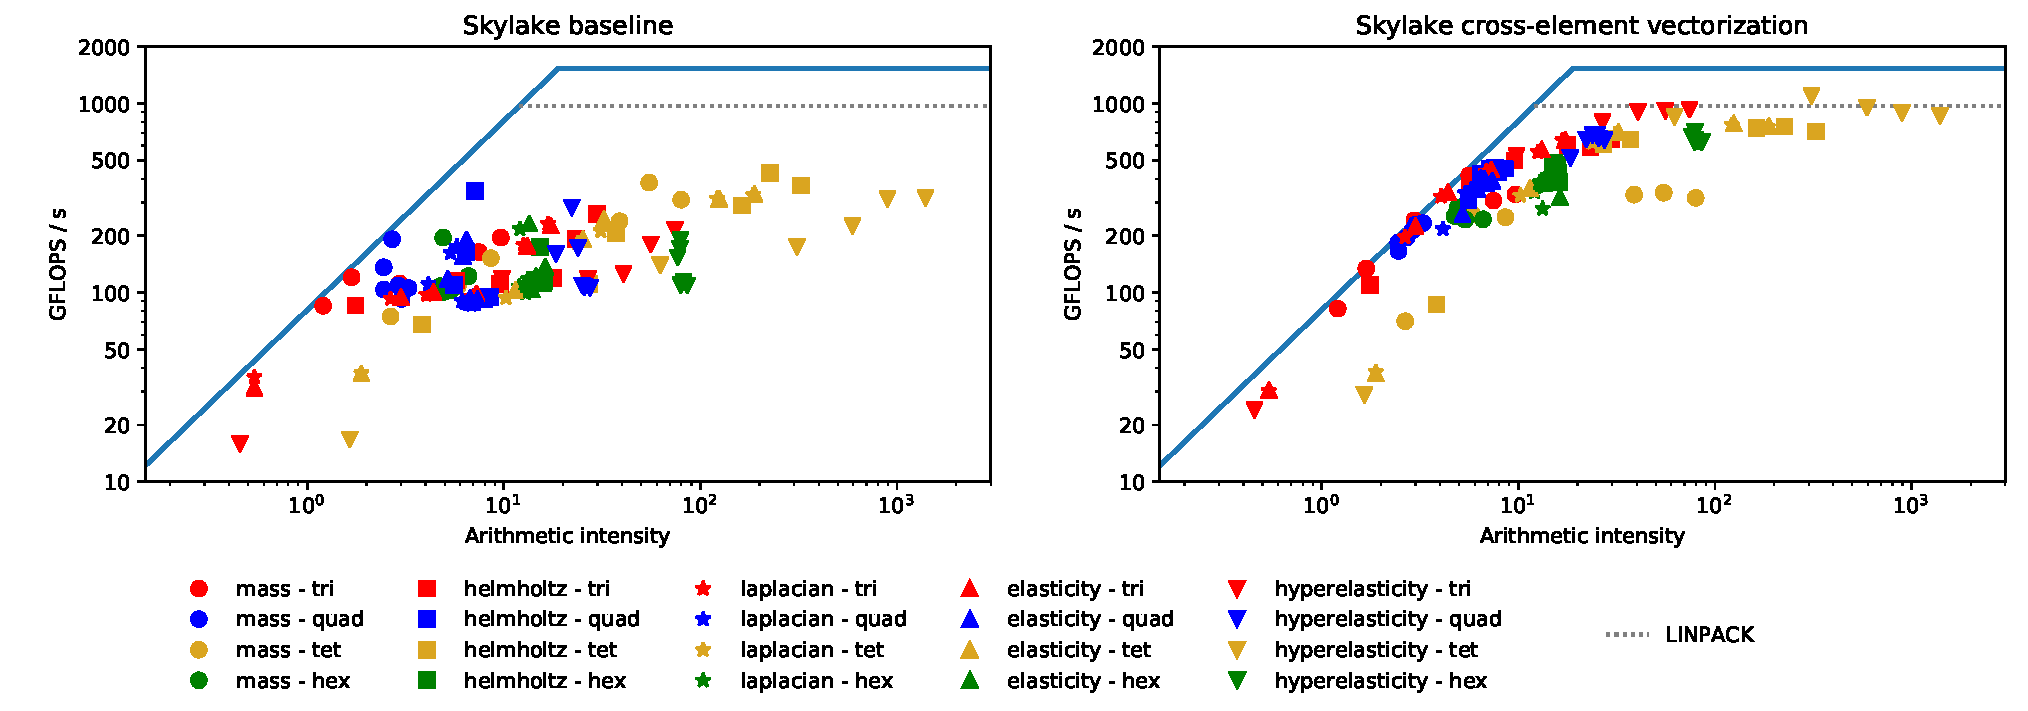
\includegraphics[width=\textwidth]{roofline-skylake}
  \end{center}
      \begin{flushright}
        {\footnotesize Sun et al.~\arxivlink{1903.08243}{cs.MS}}
      \end{flushright}
\end{frame}

\begin{frame}
  \frametitle{Idea: code generation}
  \begin{itemize}
  \item Firedrake exploits structure in extruded meshes, but nothing
    else
  \item Problem: don't want to code the cartesian product of different
    substructure components by hand
  \item Might wish to try different iteration orders, data layout
    
  \item $\Rightarrow$ develop interface for code generation
  \item Challenges: needs to look like a real mesh
  \item $\Rightarrow$ topological queries must work
  \end{itemize}
\end{frame}



\end{document}

